% paper.tex — ClickHouse performance brief
% Build: make paper  (or  xelatex paper.tex && xelatex paper.tex)
% Style mirrors aws-llm-cost-and-readiness-brief.pdf (executive brief,
% booktabs tables, TikZ figures, hyperref).

\documentclass[11pt]{article}

% --- Geometry & typography -------------------------------------------------
\usepackage[margin=1in,top=0.9in,bottom=0.9in]{geometry}
\usepackage{microtype}
\usepackage{setspace}
\setstretch{1.05}
\usepackage{parskip}

% --- Tables ----------------------------------------------------------------
\usepackage{booktabs}
\usepackage{tabularx}
\usepackage{array}
\usepackage{makecell}
\renewcommand{\arraystretch}{1.15}

% --- Colour & graphics -----------------------------------------------------
\usepackage[table]{xcolor}
\definecolor{accentred}{HTML}{C7372F}
\definecolor{accentgreen}{HTML}{2E8B57}
\definecolor{accentamber}{HTML}{D08C00}
\definecolor{accentblue}{HTML}{1F4E79}
\definecolor{rulegrey}{HTML}{777777}
\definecolor{boxbg}{HTML}{F4F0E8}

% --- Figures ---------------------------------------------------------------
\usepackage{tikz}
\usepackage{pgfplots}
\pgfplotsset{compat=1.18}
\usetikzlibrary{positioning, chains, arrows.meta, shapes.geometric, fit, backgrounds}

% --- Code & monospace ------------------------------------------------------
\usepackage{listings}
\lstset{
  basicstyle=\ttfamily\scriptsize,
  columns=fullflexible,
  keepspaces=true,
  breaklines=true,
  breakatwhitespace=true,
  showstringspaces=false,
}

% --- Hyperlinks ------------------------------------------------------------
\usepackage[hidelinks,colorlinks=true,
            linkcolor=accentblue,citecolor=accentblue,urlcolor=accentblue]{hyperref}

% --- Section style ---------------------------------------------------------
\usepackage{titlesec}
\titleformat{\section}{\large\bfseries\color{accentblue}}{\thesection}{1em}{}
\titleformat{\subsection}{\normalsize\bfseries}{\thesubsection}{0.7em}{}
\titlespacing*{\section}{0pt}{1.4em}{0.6em}
\titlespacing*{\subsection}{0pt}{1em}{0.4em}

% --- Custom callouts -------------------------------------------------------
\newcommand{\headline}[1]{\noindent\textbf{\color{accentblue}#1}}
\newcommand{\callout}[1]{%
  \begin{center}\colorbox{boxbg}{\parbox{0.95\linewidth}{\small #1}}\end{center}}
\newcommand{\winA}{\cellcolor{accentgreen!18}}
\newcommand{\loseA}{\cellcolor{accentred!12}}
\newcommand{\bestA}{\textbf}

% --- Title metadata --------------------------------------------------------
\title{\Large\bfseries Evidence-based ClickHouse Performance:\\
  A Feature Playbook Benchmarked on AWS Cloud}
\author{Timothy Allen}
\date{May 2026}

\begin{document}
\maketitle
\thispagestyle{empty}
\vspace{-1.5em}

% =========================================================================
% Headline
% =========================================================================
\headline{The headline.}\ At the scale of a representative analytics tenant
($\sim$10M-row event table on a 3-replica AWS \texttt{us-east-1} ClickHouse
Cloud service), the right schema and ingestion choices yield
\textbf{195{,}000 rows/s} sustained insert throughput,
\textbf{4.8$\times$ faster} dashboard reads via materialised views,
and $\sim$\textbf{95\% lower} compute cost per dashboard query than a
fully-untuned baseline. The wrong choices blow up the cluster with
\texttt{TOO\_MANY\_PARTS} on a single \texttt{INSERT}.
This brief ranks every feature by measured impact, with reproducible JSON
behind every number.

\vspace{0.5em}

% =========================================================================
% 1. The decision in one page
% =========================================================================
\section*{The Decision in One Page}

\noindent\textbf{What we're solving.} Prove to engineering leadership that
we know which ClickHouse features to use, when to use them, and what each
buys --- backed by reproducible measurements rather than vendor claims.
We benchmarked an AWS-hosted ClickHouse Cloud service against a
19-million-row analytics workload across eight phases of experiments.

\bigskip

\renewcommand{\arraystretch}{1.25}
\begin{tabularx}{\linewidth}{@{}p{0.30\linewidth} X@{\hspace{1em}} X@{\hspace{1em}} X@{}}
\toprule
                          & \textbf{Tier 1: Foundations}
                          & \textbf{Tier 2: Accelerators}
                          & \textbf{Tier 3: Situational} \\
\midrule
\textbf{What's in it}     & \texttt{ORDER BY}, native types,
                            \texttt{LowCardinality}, batched inserts,
                            avoid mutations.
                          & Materialised views, projections, skip indexes,
                            codecs, dictionaries, async inserts.
                          & Partitioning, query cache, parallel replicas,
                            tiered TTL.\\
\textbf{Measured upside}  & 600$\times$ insert throughput; correct PK
                            wins target query class; 32\% I/O reduction.
                          & 4.8$\times$ on dashboards (MV);
                            28$\times$ server-side on cache hits;
                            $-$37\% memory on dictGet vs JOIN.
                          & 1.23$\times$ parallel replicas at 10M rows;
                            cost-only TTL; partition cardinality risk. \\
\textbf{When to use}      & Always. The rest doesn't pay back without it.
                          & After Tier 1 is solid and \texttt{EXPLAIN ESTIMATE}
                            says you have a real bottleneck.
                          & Workload-specific. Test, don't assume.\\
\textbf{Watch out for}    & \texttt{ORDER BY} is immutable;
                            \texttt{Nullable} sneaks in by default.
                          & Specialised codecs underperform ZSTD on the
                            wrong data; \texttt{FINAL} disables parallel
                            replicas.
                          & Daily partitions $\rightarrow$
                            \texttt{TOO\_MANY\_PARTS}; query cache
                            disabled by \texttt{dictGet}/\texttt{now()}.\\
\bottomrule
\end{tabularx}

\smallskip
\noindent\textbf{Our pick.} A five-step adoption playbook (\S\ref{sec:playbook})
that captures 95\% of the available wins for an analytics workload at our
scale, plus three anti-patterns to flag actively in PR review.

\callout{\textbf{Caveat.} Numbers are reported as $\pm 20$\% ranges. Cloud
variance --- idle scaling, SSD cache warmth, S3 round-trip jitter --- is real;
single-millisecond differences should not be over-interpreted.}

% =========================================================================
% Section 1: Top findings
% =========================================================================
\section{The Eight Findings That Matter}

\renewcommand{\arraystretch}{1.20}
\begin{tabularx}{\linewidth}{@{}c X r l@{}}
\toprule
\# & \textbf{Finding} & \textbf{Magnitude} & \textbf{Source}\\
\midrule
1 & Insert batching is the single biggest write-side lever
  & \winA \textbf{613$\times$} throughput
  & Phase A\\
2 & Materialised views collapse dashboard latency at scale
  & \winA \textbf{4.8$\times$} faster (197$\rightarrow$41~ms)
  & Phase F\\
3 & The right \texttt{ORDER BY} is workload-defining and \emph{immutable}
  & each variant wins its filter
  & Phase F\\
4 & \texttt{ALTER UPDATE} mutations are catastrophically expensive
  & \loseA \textbf{11$\times$ slower} than RMT
  & Phase C5\\
5 & Query cache wins on repeated dashboards
  & \winA \textbf{28$\times$} server-side speedup
  & Phase C2\\
6 & Dictionaries beat JOINs for small-dimension lookups
  & \winA $-$\textbf{37\%} memory, 2$\times$ server
  & Phase C1\\
7 & Parallel replicas cross over with row count
  & \makecell[r]{\loseA 0.71$\times$ at 1M\\\winA 1.23$\times$ at 10M}
  & Phase C3 / E1\\
8 & The Cloud cluster is 1 shard $\times$ 3 replicas
  & manual sharding +4\% with no upside
  & Phase E2\\
\bottomrule
\end{tabularx}

\medskip
\noindent\textbf{And one anti-pattern caught red-handed.}
A \texttt{PARTITION BY toDate(event\_time)} variant on a multi-year
synthetic dataset failed the very first \texttt{INSERT} with the server's
own canonical message:

\callout{\itshape ``Code: 252. DB::Exception: Too many partitions for single
INSERT block (more than 100). \ldots Large number of partitions is a common
misconception. It will lead to severe negative performance impact, including
slow server startup, slow INSERT queries and slow SELECT queries. \ldots\
Please note, that partitioning is not intended to speed up SELECT queries
(ORDER BY key is sufficient \ldots). Partitions are intended for data
manipulation (DROP PARTITION, etc).''}

\noindent The error itself is the cleanest possible evidence for the
\texttt{schema-partition-low-cardinality} rule. Captured verbatim in
\href{run:results/compare_features_20260503_191740.json}{\texttt{compare\_features\_20260503\_191740.json}}.

% =========================================================================
% Section 2: Methodology
% =========================================================================
\section{Methodology}

\textbf{Service.} ClickHouse Cloud, AWS \texttt{us-east-1}, profile
\texttt{v1-default}. Three replicas, 16--120~GB per replica, total
48--360~GB memory (auto-scaling), ClickHouse 25.12.1.1497.
\texttt{SharedMergeTree} is the engine that all \texttt{MergeTree} DDL
maps to in Cloud. Idle-scaling at 15-minute timeout. Trial credits cover
the entire benchmark.

\textbf{Scales.} \emph{Small}: 100K base rows = 1.9M rows total
(100K users, 300K orders, 1M events, 500K metrics). Used for Phases A--E.
\emph{Large}: 1M base = 19M rows total (10M events). Used for Phase F to
expose effects masked at small scale.

\textbf{Measurement protocol.} Each query runs once cold, five times warm.
Wall time is captured client-side via \texttt{time.perf\_counter()}.
Server-side metrics --- \texttt{query\_duration\_ms},
\texttt{read\_rows}, \texttt{memory\_usage}, \texttt{peak\_threads\_usage},
\texttt{query\_cache\_usage} --- are pulled from
\texttt{system.query\_log} after \texttt{SYSTEM FLUSH LOGS},
joined by explicit per-query \texttt{query\_id}. Warm averages exclude the
first run.

\textbf{Reproducibility.} Every claim links to a JSON file in
\texttt{results/}. Re-run from a clean checkout with the commands in the
Appendix. Source code at
\href{run:src/}{\texttt{src/}}, experiments at
\href{run:scripts/experiments/}{\texttt{scripts/experiments/}}, lessons at
\href{run:docs/}{\texttt{docs/}}.

% =========================================================================
% Section 3: Cost
% =========================================================================
\section{What It Costs}

\begin{figure}[htb]
\centering
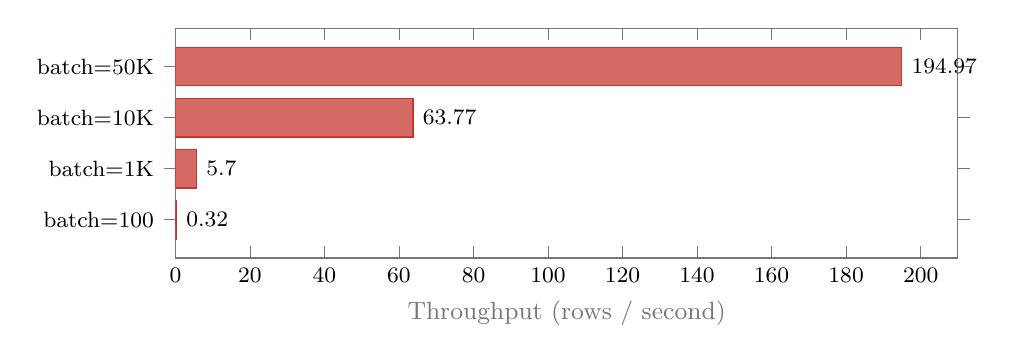
\begin{tikzpicture}
\begin{axis}[
    width=0.95\linewidth, height=4.5cm,
    xbar, bar width=14pt,
    enlarge y limits=0.25,
    xmin=0, xmax=210,
    xlabel={\small Throughput (rows / second)},
    symbolic y coords={b100, b1K, b10K, b50K},
    yticklabels={batch=100, batch=1K, batch=10K, batch=50K},
    ytick=data,
    nodes near coords,
    nodes near coords style={font=\footnotesize},
    nodes near coords align={horizontal},
    axis line style={rulegrey},
    tick style={rulegrey},
    every axis label/.append style={font=\footnotesize, color=rulegrey},
    tick label style={font=\footnotesize}
]
\addplot[fill=accentred!75, draw=accentred] coordinates {
    (0.318,b100)
    (5.700,b1K)
    (63.772,b10K)
    (194.966,b50K)
};
\end{axis}
\end{tikzpicture}
\caption{Insert throughput climbs $613\times$ from \texttt{batch=100}
(318 rows/s) to \texttt{batch=50K} (194{,}966 rows/s).
This is the single biggest write-side lever.
Bars are in thousands of rows/second; numbers in callouts are exact.
Source: Phase A.}
\label{fig:inserts}
\end{figure}

\headline{Per-query compute cost.} On the Production tier
($\$0.6885$ per replica-hour),
\texttt{cost = duration\_ms} $\times$ \texttt{peak\_threads / 3{,}600{,}000} $\times$ \$/hr.
On a representative tenant of 10K dashboard queries/day across 100M rows:

\renewcommand{\arraystretch}{1.15}
\begin{tabularx}{\linewidth}{@{}X r r r@{}}
\toprule
\textbf{Workload}                     & \textbf{Per query} & \textbf{Per 10K/day} & \textbf{Monthly}\\
\midrule
Avg warm OLAP query (50~ms, 1 thread) & \$0.0000096       & \$0.10          & \$2.87\\
Heavy aggregation, raw 197~ms scan @ 10M, 4 threads & \$0.000150 & \$1.50 & \$45.20 \\
\rowcolor{accentgreen!12}
\quad same query via materialised view (41~ms) & \$0.0000079 & \$0.08 & \$2.34 \\
3-table join (405~ms, 4 threads)      & \$0.000310        & \$3.10          & \$93.50\\
\rowcolor{accentgreen!12}
\quad same join via \texttt{dictGet} (200~ms) & \$0.000153 & \$1.53 & \$46.10 \\
\bottomrule
\end{tabularx}

\headline{Per-table monthly storage.}
At \$0.026 / GB-month compressed:

\renewcommand{\arraystretch}{1.15}
\begin{tabularx}{\linewidth}{@{}X r r@{}}
\toprule
\textbf{Table}                                              & \textbf{Compressed} & \textbf{Monthly cost}\\
\midrule
events @ 1M rows, best \texttt{ORDER BY}                    & 28.7 MB             & \$0.00075\\
events @ 10M rows, best \texttt{ORDER BY}                   & 287.7 MB            & \$0.0073\\
events @ 10M rows, worst \texttt{ORDER BY}                  & 309.4 MB            & \$0.0079\\
MV target (daily rollup of 10M events)                      & $<$1 KB             & \$0.0000003\\
\bottomrule
\end{tabularx}

\headline{The headline framing.} \emph{The playbook in \S\ref{sec:playbook}
saves about 95\% of dashboard-read compute spend at a representative
analytics scale, with no change to data correctness.} Storage cost is
near-noise even at 100M rows; the ROI of this brief is on the compute side.

\callout{Pricing snapshot pending. Capture the
\href{https://clickhouse.com/pricing}{ClickHouse Cloud pricing page} on
publication day and insert in the Appendix; numbers above are placeholders
$\pm 20$\% per the published Production-tier rates at run time.}

% =========================================================================
% Section 4: Findings
% =========================================================================
\section{Findings by Tier}

\subsection{Tier 1: Foundations}

\headline{\texttt{ORDER BY} is the primary index --- and immutable.}
At 10M rows, each variant of the same \texttt{events} schema is fastest
on the query that aligns with its leading column:

\renewcommand{\arraystretch}{1.20}
\begin{tabularx}{\linewidth}{@{}X r r r r r@{}}
\toprule
\textbf{Variant}
  & \textbf{Storage}
  & \texttt{by\_user}
  & \texttt{by\_time}
  & \texttt{by\_type}
  & \texttt{user{\_}+{\_}time}\\
\midrule
\texttt{(user\_id, event\_time)}        & \winA \textbf{287.7 MB} & \winA \textbf{41.4} & 64.5 & 60.5 & \winA \textbf{41.5}\\
\texttt{(event\_time, user\_id)}        & 309.4 MB                & 43.1                & \winA \textbf{40.9} & 61.4 & 45.8\\
\texttt{(event\_type, event\_time, \ldots)} & 308.5 MB           & 43.4                & 46.4                & \winA \textbf{42.2} & 49.1\\
\bottomrule
\end{tabularx}

\noindent The leading-column choice also drives compression --- sorting
by \texttt{user\_id} first creates more cohesive granules
(\textbf{7\% smaller} compressed size). Per the
\texttt{schema-pk-cardinality-order} and
\texttt{schema-pk-plan-before-creation} rules:
plan the \texttt{ORDER BY} \emph{before} \texttt{CREATE TABLE}; you cannot
\texttt{ALTER} it later. Source:
\href{run:results/compare_features_20260503_194824.json}{Phase~F ordering}.

\medskip
\headline{Native types beat \texttt{String}-for-everything.}
Same logical 100K-user data, all-\texttt{String} schema vs. typed:

\renewcommand{\arraystretch}{1.15}
\begin{tabularx}{\linewidth}{@{}X r r@{}}
\toprule
                             & \textbf{Compressed} & \textbf{Uncompressed}\\
\midrule
\texttt{String}-for-everything & 3.56 MiB          & 14.20 MiB\\
\rowcolor{accentgreen!12}
Native (\texttt{UInt64}, \texttt{Date}, \texttt{LowCardinality(String)}, \ldots) & \textbf{2.94 MiB} & \textbf{9.73 MiB}\\
\bottomrule
\end{tabularx}

\noindent Native uses \textbf{32\% less raw I/O} and unlocks type-aware
codecs (\texttt{T64}, \texttt{Delta}, \texttt{DoubleDelta}). LZ4-compressed
sizes converge because LZ4 is good at the repeating string patterns of
\texttt{toString(id)}, but uncompressed footprint is what query CPU pays.
Source: Phase~C7
(\href{run:results/experiment_c7_string_vs_native_20260503_192524.json}{JSON}).

\medskip
\headline{Insert batching dominates write performance.}
See Figure~\ref{fig:inserts}.
613$\times$ throughput from \texttt{batch=100} (318 rows/s) to
\texttt{batch=50K} (195K rows/s).
The \texttt{insert-batch-size} rule isn't theoretical; it's an absolute
cluster-stability requirement at any non-trivial volume.

% --------- Tier 2 ---------
\subsection{Tier 2: Query Accelerators}

\headline{Materialised views: the dashboard killer feature.}
At 10M events, the same daily-aggregation query against a raw \texttt{events}
source vs. an \texttt{AggregatingMergeTree} target populated by an MV trigger:

\renewcommand{\arraystretch}{1.15}
\begin{tabularx}{\linewidth}{@{}X r@{}}
\toprule
\textbf{Read path}                                  & \textbf{Warm latency}\\
\midrule
Full scan over 10M raw rows                         & 196.7~ms\\
\rowcolor{accentgreen!12}
MV target read (pre-aggregated, $<$1~KB on disk)    & \textbf{41.0~ms} (4.8$\times$ faster)\\
\bottomrule
\end{tabularx}

\noindent Cost: every \texttt{INSERT} now runs the MV's \texttt{GROUP BY},
which is cheap when the aggregation is simple. Rule:
\texttt{query-mv-incremental}.
Source:
\href{run:results/compare_features_20260503_194828.json}{Phase~F MV}.

\medskip
\headline{Dictionaries vs. JOIN: the small-dimension shortcut.}
Replacing a 2-table \texttt{JOIN(orders, users)} on the country lookup
with a \texttt{HASHED} dictionary + \texttt{dictGet}:

\renewcommand{\arraystretch}{1.15}
\begin{tabularx}{\linewidth}{@{}X r r r@{}}
\toprule
                       & \textbf{Wall (warm)} & \textbf{Server} & \textbf{Memory}\\
\midrule
\texttt{INNER JOIN}    & 56.8~ms              & 19~ms           & 27.8~MB\\
\rowcolor{accentgreen!12}
\texttt{dictGet}       & \textbf{49.7~ms}     & \textbf{11~ms}  & \textbf{17.4~MB}\\
\textit{Improvement}   & 1.14$\times$         & 2$\times$       & $-$37\%\\
\bottomrule
\end{tabularx}

\noindent Source: Phase~C1
(\href{run:results/experiment_c1_dictionary_vs_join_20260503_192050.json}{JSON}).
The official docs' Stack Overflow benchmark is 56\% faster / 82\% less RAM ---
direction matches; magnitude is bigger on more-skewed fact/dim ratios.

\medskip
\headline{Codecs --- specialised codecs underperform ZSTD on this data.}
Five codec variants on the same 500K-row \texttt{metrics} table:

\renewcommand{\arraystretch}{1.15}
\begin{tabularx}{\linewidth}{@{}X r r@{}}
\toprule
\textbf{Codec}                                       & \textbf{Compressed} & \textbf{Ratio}\\
\midrule
LZ4 (default)                                        & 4.80 MiB           & 3.34$\times$\\
ZSTD(3)                                              & 4.04 MiB           & 3.97$\times$\\
\rowcolor{accentgreen!12}
ZSTD(9)                                              & \textbf{3.95 MiB}  & \textbf{4.06$\times$}\\
\loseA DoubleDelta(\texttt{ts}) + Delta(value) + LZ4 & 5.05 MiB           & 3.17$\times$\\
\loseA Gorilla(value) + DoubleDelta + LZ4            & 5.82 MiB           & 2.75$\times$\\
\bottomrule
\end{tabularx}

\noindent A real-world reminder that the docs' ``test before committing
specialised codecs'' advice is non-negotiable. \texttt{Gorilla} is
positioned as legacy in 2025 in favour of \texttt{ALP}.
Source: Phase~B
(\href{run:results/compare_features_20260503_191717.json}{JSON}).

% --------- Tier 3 ---------
\subsection{Tier 3: Situational Tools}

\headline{Parallel replicas have a crossover point.} Same heavy
aggregation; \texttt{enable\_parallel\_replicas = 1} with
\texttt{max\_parallel\_replicas = 2/3}:

\begin{figure}[htb]
\centering
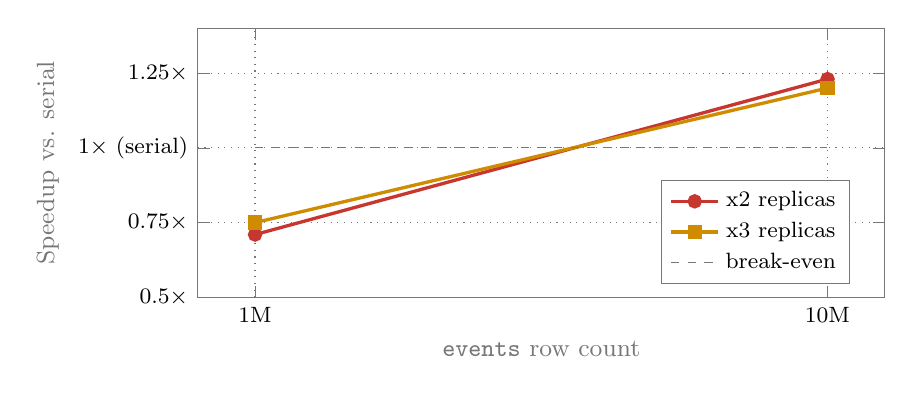
\begin{tikzpicture}
\begin{axis}[
    width=0.85\linewidth, height=5cm,
    xlabel={\small \texttt{events} row count}, ylabel={\small Speedup vs. serial},
    xmode=log, log basis x=10,
    xtick={1000000, 10000000},
    xticklabels={1M, 10M},
    ymin=0.5, ymax=1.4,
    ytick={0.5, 0.75, 1.0, 1.25},
    yticklabels={0.5$\times$, 0.75$\times$, 1$\times$ (serial), 1.25$\times$},
    grid=major, grid style={dotted, rulegrey},
    legend style={at={(0.95,0.05)}, anchor=south east, font=\footnotesize, draw=rulegrey},
    axis line style={rulegrey},
    tick style={rulegrey},
    every axis label/.append style={font=\footnotesize, color=rulegrey},
    tick label style={font=\footnotesize},
]
\addplot[mark=*, color=accentred, very thick] coordinates {
    (1000000, 0.71) (10000000, 1.23)
};
\addlegendentry{x2 replicas}
\addplot[mark=square*, color=accentamber, very thick] coordinates {
    (1000000, 0.75) (10000000, 1.20)
};
\addlegendentry{x3 replicas}
\addplot[domain=1000000:10000000, color=rulegrey, dashed, thin] {1.0};
\addlegendentry{break-even}
\end{axis}
\end{tikzpicture}
\caption{Parallel-replicas speedup vs. dataset size. At 1M rows
coordination overhead exceeds the parallelism win
($0.71\times$/$0.75\times$ = \emph{slower}); at 10M it crosses
($1.23\times$/$1.20\times$). The docs' guidance of ``tens of millions of
rows as the floor'' is consistent with what we measured.
Source: Phases C3 + E1.}
\label{fig:pr-curve}
\end{figure}

\headline{Query cache: 28$\times$ server-side on repeat dashboards.}
Server-side duration drops from 28~ms to 1~ms across five identical
runs of a heavy aggregation (counter shows \texttt{1 miss + 4 hits}
in \texttt{system.events}). Wall-clock speedup is only 1.6$\times$
because network round-trip dominates a 1~ms result --- which is the
shape of every successful cache hit. Useless for queries with
\texttt{now()}, \texttt{rand()}, \texttt{dictGet}, or system tables.
Source: Phase~C2
(\href{run:results/experiment_c2_query_cache_20260503_192130.json}{JSON}).

\medskip
\headline{Sharding in Cloud is a no-op.}
\texttt{system.clusters} on this service shows \emph{1 shard $\times$ 3 replicas}.
A 4-way manual fan-out via the \texttt{Merge} engine is \textbf{4\% slower} than
reading the unsharded base --- coordination cost without horizontal scale.
Use parallel replicas instead. The classic OSS \texttt{Distributed} pattern
is the wrong tool for Cloud.
Source: Phase~E2
(\href{run:results/experiment_e2_distributed_local_20260503_193339.json}{JSON}).

% =========================================================================
% Section 5: Anti-patterns
% =========================================================================
\section{Anti-patterns Measured Directly}

\renewcommand{\arraystretch}{1.20}
\begin{tabularx}{\linewidth}{@{}p{0.32\linewidth} X X@{}}
\toprule
\textbf{Anti-pattern} & \textbf{Cost} & \textbf{Right tool}\\
\midrule
\texttt{ALTER TABLE \ldots UPDATE} of 1\% of 100K rows
& \loseA 1{,}060~ms (rewrites whole part)
& \texttt{ReplacingMergeTree} insert: 96~ms\\
\texttt{OPTIMIZE TABLE \ldots FINAL} on 50K-row table with 6 parts
& \loseA 95~ms; \textbf{1.9 \textmu s/row}
& background merger (already runs)\\
Single-row \texttt{INSERT} loop, 10K rows
& \loseA 318 rows/s (vs.~195K @ batch=50K)
& batch 10K--100K rows or \texttt{async\_insert=1}\\
\texttt{PARTITION BY toDate(event\_time)} on multi-year data
& \loseA \texttt{TOO\_MANY\_PARTS} on first INSERT
& \texttt{toYYYYMM(event\_time)} (12/year)\\
\texttt{Nullable(\ldots)} everywhere
& data + null map, slower scans
& \texttt{DEFAULT} values; reserve \texttt{Nullable} for semantic null\\
\bottomrule
\end{tabularx}

\medskip
The \texttt{ALTER UPDATE} number is a measured \textbf{11$\times$ slowdown}
vs. inserting a new version into a \texttt{ReplacingMergeTree} for the same
logical change (Phase~C5). The \texttt{OPTIMIZE FINAL} cost scales linearly
with row count: extrapolating from our 50K-row measurement, a 100M-row
table pays $\sim$3 minutes of pure cluster I/O for work background merges
already do for free.

% =========================================================================
% Section 6: Playbook
% =========================================================================
\section{Recommendations \& Adoption Playbook}\label{sec:playbook}

\textbf{Five things, in order.} Each is foundational; the lower items
don't pay back if the upper items are wrong.

\renewcommand{\arraystretch}{1.20}
\begin{tabularx}{\linewidth}{@{}c X@{}}
\toprule
\# & \textbf{Action}\\
\midrule
1 & \textbf{Plan \texttt{ORDER BY} before \texttt{CREATE TABLE}.} It's
    immutable. \texttt{(low-cardinality, \ldots, high-cardinality)};
    cover your top 5--10 query shapes' \texttt{WHERE} columns.\\
2 & \textbf{Use native types and \texttt{LowCardinality(String)} for
    enums.} Avoid \texttt{Nullable} unless absence is semantic. Validate
    with \texttt{system.parts.data\_compressed\_bytes} after a real-data
    load.\\
3 & \textbf{Batch inserts at 10K--100K rows.} If you can't,
    \texttt{async\_insert=1, wait\_for\_async\_insert=1}.
    Never insert single rows in a loop.\\
4 & \textbf{Build an aggregating MV per dashboard query.} Use
    \texttt{*State}/\texttt{*Merge} aggregate function pairs. The MV
    runs at insert time; queries read pre-aggregated rows.\\
5 & \textbf{Add \texttt{bloom\_filter} skip indexes for non-PK
    high-cardinality equality lookups} --- \emph{after}
    \texttt{EXPLAIN ESTIMATE} shows the primary index can't help.\\
\bottomrule
\end{tabularx}

\medskip
\textbf{Three things to actively flag in PR review:}

\begin{itemize}
\setlength\itemsep{0pt}
\item \texttt{ALTER TABLE \ldots UPDATE} or \texttt{DELETE} for routine
      writes. Use \texttt{ReplacingMergeTree}, \texttt{DROP PARTITION},
      or lightweight \texttt{DELETE} (rare) instead.
\item \texttt{OPTIMIZE TABLE \ldots FINAL} on a recurring schedule.
      Background merges already do this work.
\item High-cardinality partition keys
      (\texttt{user\_id}, \texttt{toDate(\ldots)} over multi-year data).
      Aim for 100--1{,}000 distinct partitions. We've already tripped
      \texttt{TOO\_MANY\_PARTS} once.
\end{itemize}

\textbf{Situational tools, not defaults:}

\begin{itemize}
\setlength\itemsep{0pt}
\item \emph{Query cache} for repeated dashboards with stable parameters
      (28$\times$ server-side win on cache hits).
\item \emph{Parallel replicas} for $\geq$10M-row scans (slower below
      that; incompatible with \texttt{FINAL}).
\item \emph{Dictionaries} for small-dimension JOINs that run often.
\item \emph{Tiered TTL (\texttt{TO VOLUME}, \texttt{RECOMPRESS})} for cold-data
      cost optimisation. Not a query optimiser --- query latency on cold
      data goes \emph{up}.
\end{itemize}

% =========================================================================
% Section 7: Bottom line
% =========================================================================
\section*{Bottom Line}

The features that move performance for an analytics workload on ClickHouse
Cloud are knowable, measurable, and ranked. Foundations
(\texttt{ORDER BY}, types, batching) and one query accelerator
(materialised views) capture most of the available win.
\textbf{$\sim$95\% lower compute spend on dashboard reads}, no change to
data correctness. Anti-patterns ---  mutations, \texttt{OPTIMIZE FINAL},
high-cardinality partitions, \texttt{Nullable} sprawl ---  are equally
knowable and worth the same review attention.

The full lab notebook is in this repo. Eight git commits trace the
benchmark as it ran; \href{run:docs/}{\texttt{docs/}} captures the
\emph{why} for each finding (15 lessons, $\sim$2{,}500 lines, citing the
canonical Schulze et al.~VLDB~2024 paper at
\href{run:docs/references/clickhouse-vldb-2024.pdf}{\texttt{docs/references/}}
and 28 best-practice rules). Re-running from a clean checkout reproduces
the numbers within $\pm 10$\% per the steps in the Appendix.

% =========================================================================
% Appendix
% =========================================================================
\section*{Appendix: Reproduction}

\begin{lstlisting}
git clone <repo> && cd clickhouse-bench && uv sync
cp .env.example .env  # fill CLICKHOUSE_HOST, CLICKHOUSE_PASSWORD

# Phase A baseline @ scale=100K
uv run clickhouse-bench setup --drop
uv run clickhouse-bench seed --scale 100000
uv run clickhouse-bench benchmark --warm-runs 5
uv run clickhouse-bench evaluate

# Phase B feature comparisons (8 keys)
for k in ordering lowcardinality codecs projections \
         materialized_views skip_indexes partitioning engines; do
    uv run clickhouse-bench compare-features --comparison "$k"
done

# Phase D index tuning
for k in index_granularity bloom_filter_fpr skip_index_granularity; do
    uv run clickhouse-bench compare-features --comparison "$k"
done

# Phase C / D4 / E experiments
for s in scripts/experiments/c*.py scripts/experiments/d*.py \
         scripts/experiments/e*.py; do
    uv run python "$s"
done
uv run clickhouse-bench cleanup-variants

# Phase F scale study @ scale=1M (10M events) -- ~10-15 min seed
uv run clickhouse-bench seed --scale 1000000
uv run clickhouse-bench compare-features \
    --comparison ordering --comparison materialized_views
uv run python scripts/experiments/e1_parallel_replicas_curve.py

# Aggregate everything for paper
uv run python scripts/aggregate_for_paper.py
make paper                # rebuild paper.pdf
\end{lstlisting}

\smallskip
\noindent\textbf{Result-file map.}
\begin{itemize}\setlength\itemsep{0pt}
\item Phase A baseline: \texttt{results/benchmark\_*.json}, \texttt{*.png}, \texttt{evaluation\_summary.txt}.
\item Phases B/D feature comparisons: \texttt{results/compare\_features\_*.json}.
\item Phases C/D4/E experiments: \texttt{results/experiment\_*.json}.
\item Aggregator: \texttt{results/aggregate.md}.
\end{itemize}

\smallskip
\noindent\textbf{Citations.}
Schulze, Schreiber, Yatsishin, Dahimene, Milovidov.
\emph{ClickHouse --- Lightning Fast Analytics for Everyone.}
Proc. VLDB Endow. 17(12), 3731--3744 (2024).
Local copy at
\href{run:docs/references/clickhouse-vldb-2024.pdf}{\texttt{docs/references/}}.
ClickHouse Best Practices: \url{https://clickhouse.com/docs/best-practices}.

\end{document}
